\documentclass[12pt,a4paper]{article}
\usepackage{mwe}
\usepackage{graphicx} % Required for inserting images
\usepackage{xcolor}
\usepackage[nottoc,numbib]{tocbibind}
\usepackage{listings}
\usepackage{hyperref}
\usepackage{indentfirst}
\usepackage{tabularx}
\lstdefinestyle{myCustomMatlabStyle}{
  language=Matlab,
  numbers=left,
  stepnumber=1,
  numbersep=10pt,
  tabsize=4,
  showspaces=false,
  showstringspaces=false
}
\lstset{
basicstyle=\fontsize{8}{8}
\selectfont\ttfamily,
style=myCustomMatlabStyle,
breaklines=true}
\hypersetup{
    colorlinks=true,
    linkcolor=blue,
    filecolor=magenta,
    urlcolor=cyan,
    pdftitle={Overleaf Example},
    pdfpagemode=FullScreen,
    }

\urlstyle{same}

\begin{document}
\begin{titlepage}
	\centering
	{\LARGE \textsc{Universitatea de Vest din Timisoara}\par}
	\vspace{1cm}
	{\huge\bfseries Testarea modelelor acasxu folosind nnenum și alpha beta\par}
	\vspace{2cm}
	{\Large\itshape
					Bogdan Topliceanu \\
					Mihai Bîzdoacă\\
					Mihai Oșan \\
					Mihai Vicol\par}
	\vfill
	supervised by\par
	Madalina Erascu

	\vfill

% Bottom of the page
	{\large \today\par}
\end{titlepage}

\section{Introducere}
Verificarea rețelelor neuronale reprezintă un pas important în asigurarea funcționalității corespunzătoare a acestora.
Întrucât detectarea și prevenirea coliziunilor aeriene este o temă relevantă în cadrul
verificării de rețele neuronale am optat pentru utilizarea setului de date ACAS Xu. Pentru a face
această verificare este necesară folosirea de tool-uri specializate pentru a evalua corectitudinea, siguranța și performanța acestora.
Procesul de verificare a setului este realizat folosind tool-urile: Alpha-Beta-CROWN și Nnenum(Neural Network Enumeration). Am ales aceste instrumente datorită popularității acestora
precum și a preciziei, și a rezultatelor satisfăcătoare din anii precedenți ai competiției.
Întocmirea acestui raport are ca scop documentarea facilă a instalării, utilizării și a rezultatelor obținute prin intermediul a două
tool-uri disponibile în cadrul competiției. Rezultatele noastre vor fi ulterior comparate cu rezultatele oficiale ale competiției.
\section{Dataset}

\subsection{ACAS XU}

ACAS Xu se referă la un set de benchmark-uri legate de verificarea rețelelor neurale, în special în contextul sistemelor de evitare a coliziunilor în aviație. ACASXu este o abreviere pentru "Aircraft Collision Avoidance System - Xu". Acest ansamblu de teste este conceput pentru a evalua robustețea și siguranța modelelor de învățare automată utilizate în sistemele de evitare a coliziunilor aeriene.\cite{acasxu}

Utilizează o combinație de senzori pentru a detecta aeronavele din apropiere, inclusiv transpondere ADS-B (dispozitiv ce ofera informatii precum poziție, viteză, altitudine etc), radar și senzori EO/IR (Electro-Optical si Infrared, adica imagini vizuale si termice). Sistemul folosește apoi o logică de decizie bazată pe un model Markov pentru a genera instrucțiuni de manevră pentru a evita coliziunea.

Logica de decizie a ACAS Xu funcționează prin calcularea probabilității de coliziune între UAS și aeronavele din apropiere. Dacă probabilitatea de coliziune este mai mare decât o anumită valoare prag, ACAS Xu va genera instrucțiuni de manevră pentru a evita coliziunea.

Instrucțiunile de manevră sunt generate folosind o abordare de minimizare a costurilor. Această abordare încearcă să găsească instrucțiunile care vor minimiza riscul de coliziune, în timp ce vor minimiza și impactul asupra aeronavei UAS.

O descriere mai detaliată:

\begin{itemize}
  \item
    Detectarea aeronavelor în apropiere: ACAS Xu utilizează o combinație de senzori pentru a detecta aeronavele din apropiere.
  \item Estimarea stării aeronavelor: ACAS Xu utilizează informațiile de la senzori pentru a estima starea aeronavelor din apropiere. Acestea includ poziția, viteza și direcția aeronavelor.
  \item Calcularea probabilității de coliziune: ACAS Xu utilizează modelul Markov pentru a calcula probabilitatea de coliziune între UAS și aeronavele din apropiere.
   \item Generarea instrucțiunilor de manevră: ACAS Xu utilizează abordarea de minimizare a costurilor pentru a genera instrucțiuni de manevră care vor minimiza riscul de coliziune.
\end{itemize}
\begin{figure}
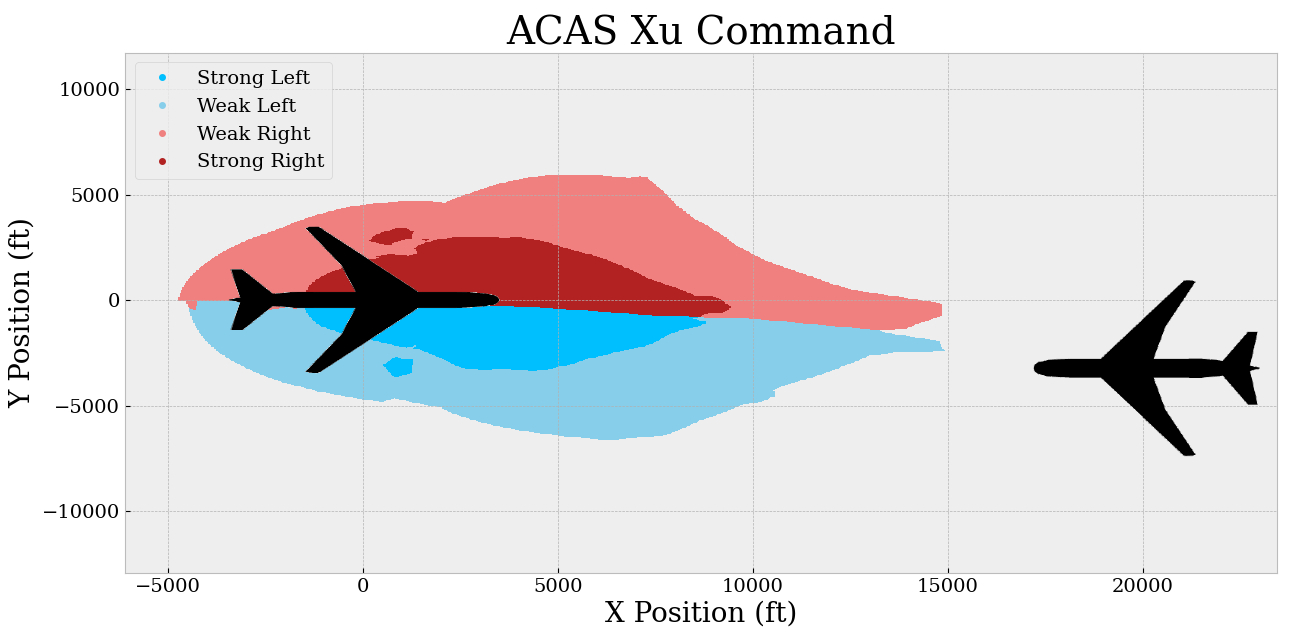
\includegraphics[scale=0.4]{headon.png}
\caption{comenzi evitare coliziune}
\end{figure}

\subsection{Structura datelor}

ONNX este un format pentru fișierele ce reprezintă modele de învățare automată, conținând astfel arhitectura unei rețele neurale. Această arhitectură arată modul în care rețeaua procesează și analizează datele în mai multe straturi. Stratul de intrare primește datele, asupra cărora vor fi efectuate o serie de calcule matematice (cum ar fi înmulțirea, adunarea, scăderea etc.). Rezultatele reprezintă predicții sau clasificări, în funcție de scopul rețelei, și fac parte din stratul de ieșire.

VNN-LIB este un format pentru specificarea proprietăților și cerințelor pe care o rețea neurală ar trebui să le îndeplinească. Datele primite în stratul de intrare, constrangerile si/sau conditiile care ar trebui indeplinite in timpul verificarii retelei sunt reprezentate în acest format.

În benchmark-ul ACAS Xu, fișierele ONNX definesc modul în care rețeaua procesează datele de intrare, care sunt specificate în fișierele VNN-LIB. Rezultatele sunt apoi evaluate în raport cu condițiile stabilite alături de informațiile furnizate. Aceste condiții sunt concepute pentru a asigura comportamentul sigur al rețelei în scenariile care ar putea fi întâlnite în contextele reale de aviație. Dacă ieșirea îndeplinește constrângerile specificate, rețeaua este considerată că funcționează corespunzător în acel scenariu; în caz contrar, indică o posibilă problemă sau eșec în îndeplinirea cerințelor.
\section{Tool-uri}
Există mai multe instrumente și framework-uri specializate pentru verificarea rețelelor neuronale. Acestea sunt utilizate pentru a evalua robustețea, corectitudinea și alți factori critici în funcționarea rețelelor neuronale.

\subsection{Nnenum}
Nnenum (Neural Network Enumeration Tool) este un instrument pentru verificarea rețelelor neuronale, în special a celor cu funcții de activare ReLU (Rectified Linear Unit). Nnenum se distinge prin abilitatea sa de a efectua verificări eficiente, folosind abstracții optimizate pentru a îmbunătăți viteza de verificare, fără a piede din acuratețea răspunsurilor.\cite{nnenum}

\subsubsection{Instalare Nnenum}

Pentru a facilita utilizarea sa, nnenum oferă posibilitatea de a utiliza Docker pentru instalare, izolând complexitatea configurării în containere auto-suficiente.

Primul pas în utilizarea Docker este instalarea acestuia. Descărcarea se realizează de pe site-ul oficial \url{https://www.docker.com}.

Înainte de a rula Dockerfile-ul pentru nnenum, este necesar să clonăm repozitorul acestuia. Acest pas asigură că avem cea mai recentă versiune a codului și toate fișierele necesare pentru instalare. Repozitorul: \url{https://github.com/stanleybak/nnenum/tree/master}.

Avand Dockerfile-ul, următorul pas este construirea imaginii Docker. Acest proces se realizează în terminal, executând comanda:
\begin{lstlisting}[language=bash]
    docker build . -t nnenum\_image
\end{lstlisting}

Această comandă crează un director ”work” în interiorul Doker-ului în care sunt copiate toate fisierele din repozitor, după care sunt înstalate librăriile de care nnenum are nevoie (aflate în ”requirements.txt”).

Urmează rularea nnenum într-un container Docker. Acest pas este realizat printr-o simplă comandă care pornește un container bazat pe imaginea nnenum:
\begin{lstlisting}[language=bash]
    docker run nnenum\_image bash
\end{lstlisting}

Imaginea creată rulează la final un script shell (run\_tests.sh) în care putem apela induvidual fiecare test din benchmark, spre exemplu:

\vspace{2mm}

\begin{lstlisting}[language=bash]
#!/bin/bash -e
echo "Running tests one by one. If 'Passed all tests.' is printed at then end, then we were successful."
python3 -m nnenum.nnenum examples/acasxu/data/ACASXU_run2a_1_1_batch_2000.onnx examples/acasxu/data/prop_1.vnnlib
echo "Passed all tests."
\end{lstlisting}
sau putem verifica toate testele din benchmark prin:

\begin{lstlisting}[language=bash]
#!/bin/bash -e
echo "Running ACAS Xu benchmarks using acasxu_all.py"
cd examples/acasxu
python3 acasxu_all.py > result_acasxu_all.txt
echo "All ACAS Xu benchmarks have been executed."
\end{lstlisting}

\subsubsection{Rezultate Nnenum pentru AcasXU}

Testele au fost realizate pe un dispozitiv MacBook Pro 13 2020 cu procesor M1 și 8GB RAM. Pentru testare s-a folosit versiunea care verifica toate testele de run\_tests.sh.

În urma rulării s-au obținut următorul set de rezultate (aflate în fisierul ”full\_acasxu.dat”):

\[
\begin{array}{|c|c|c|c|}
\hline
 onnx & proprietate & rezultat  & timp  \\
\hline
1\_1&	1&	holds&	1.7305238750013814\\
1\_2&	1&	holds&	1.4748255840004276\\
1\_3&	1&	holds&	1.5281753340004798\\
1\_4&	1&	holds&	1.4214602920001198\\
...&...&...&...\\
1\_1&	2&	holds&	1.7493573749998177\\
1\_2	&	2&	violated&	1.6237783759988815\\
1\_3&	2&	violated&	1.855259958998431\\
...&...&...&...\\
2\_9&	8&	violated&	0.6185222500007512\\
3\_3&	9&	holds&	2.9630538760011405\\
4\_5&	10&	holds&	0.8966264169994247\\
\hline
\end{array}
\]

Pentru rezultate, termenul "holds" reprezintă faptul că rețeau este ”Safe”, iar ”violateted” este ”Unsafe”. Pentru rețelele nesigure pentru o anumită proprietate se generează și se afișează și un contraexemplu. Toate contraexemplele, împreună cu rezultatele complete ale testelor, sunt salvate în fisierul ”result\_acasxu\_all.txt”. Exemplu pentru modelul 1\_4 cu proprietateaa 2:

\begin{lstlisting}[language=bash]
Result: network is UNSAFE with confirmed counterexample in result.cinput and result.coutput
Input: [0.6301487684249878, -0.009191256947815418, 0.4637353718280792, 0.5, -0.44999998807907104]
Output: [-0.016746846958994865, -0.018340758979320526, -0.01793942041695118, -0.017191750928759575, -0.017659002915024757]
\end{lstlisting}

\begin{tabularx}{1.1\textwidth}{ | >{\centering\arraybackslash}X | >{\centering\arraybackslash}X | X | X | X | X | X | }
  \hline
   Tool & Verified & Falsified & Fastest & Penalty & Score & Percent \\
\hline
   Nnenum & 139 & 47 & 0 & 0 & 1860 & 100 \\
\hline
\end{tabularx}
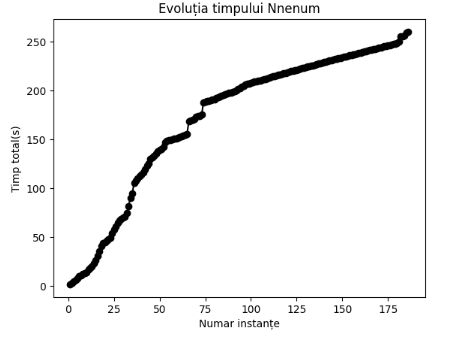
\includegraphics[]{timp_nn.png}


\vspace{5mm}
\subsection{Alpha-Beta-Crown}
Alpha-Beta-CROWN reprezintă un sistem de verificare open-source pentru rețele neuronale, fundamentat pe un algoritm eficient de propagare a limitelor și tehnici de branch-and-bound. Acesta oferă o abordare robustă pentru evaluarea și asigurarea proprietăților rețelelor neuronale, fiind construit pe principii care integrează atât alpha, cât și beta, în vederea optimizării performanțelor. \cite{Alpha-Beta-CROWN}

CROWN acționează ca un sistem general specializat în certificarea robusteței rețelelor neuronale. Adaptându-se la funcțiile generale de activare pentru anumite puncte de date de intrare, CROWN oferă o metodologie extinsă pentru a evalua și asigura comportamentul corect al rețelelor în fața perturbațiilor.

Beta-CROWN aduce în discuție o metodă inovatoare de propagare a limitelor, capabilă să codifice în totalitate diviziunile neuronale. Acest lucru este realizat prin intermediul parametrilor optimizabili Beta, construiți cu precădere din spațiul primal sau dual.

Alpha-CROWN, în schimb, este conceput pentru a aborda scenarii de verificare incomplete. Integrând o limită CROWN optimizată, Alpha-CROWN oferă un echilibru între acuratețea verificării și eficiența computatională.

În ansamblu, aceste componente alpha, beta și CROWN constituie un ecosistem complex și flexibil pentru verificarea și certificarea rețelelor neuronale, contribuind astfel la avansarea în înțelegerea și utilizarea acestora în aplicații variate.
\subsubsection{Instalare Alpha-Beta-Crown}
Pașii pentru instalarea și rularea Alpha,Beta-CROWN:
Clonăm repository-ul Alpha,Beta-CROWN de pe GitHub, inclusiv submodulul autoLiRPA, dar si vnncomp2023\_Benchmark:
\begin{lstlisting}
git clone --recursive https://github.com/Verified-Intelligence/alpha-beta-CROWN.git
cd alpha-beta-CROWN
\end{lstlisting}
Se recomandă folosirea unui mediu virtual pentru a evita conflicte între dependențe. Astfel, se elimină un mediu existent și se creeaza unul nou pentru Alpha,Beta-CROWN:
\begin{lstlisting}
conda deactivate   #Dezactiveaza mediul curent (daca este activ)
conda env remove --name alpha-beta-crown   #Elimina mediu existent, daca este cazul
conda env create -f complete_verifier/environment.yaml --name alpha-beta-crown   #Creeaza si instaleaza dependente in noul mediu
conda activate alpha-beta-crown   Activeaza noul mediu
\end{lstlisting}
În contextul programării pe GPU (unitate de procesare grafică), CUDA reprezintă un model de programare și un set de instrumente dezvoltate de către NVIDIA. CUDA permite dezvoltatorilor să utilizeze puterea de calcul a GPU-urilor NVIDIA pentru a accelera anumite tipuri de sarcini, cum ar fi calculele intensive, în special cele din domeniul științific și al învățării automate (machine learning).
Pentru rulare se utilizeaza scriptul abcrown.py. Toți parametrii sunt definiți într-un fișier de configurare YAML pentru a defini condițiile sub care se efectuează verificarea și a adapta algoritmul la specificul problemei sau setului de date utilizat. Pentru a verifica robustețea retelei AcasXU, folosim:
\begin{lstlisting}
conda activate alpha-beta-crown  # Activeaza mediu Conda
cd complete_verifier
python abcrown.py --config complete_verifier/exp_configs/vnncomp23/acasxu.yaml
\end{lstlisting}

\subsubsection{Rezultate Alpha-Beta-Crown pentru AcasXU}
Testele au fost realizate pe un dispozitiv ASUS TUF A15 2020 cu placa video Nvidia GTX 1660ti  și 16GB RAM.
\\
\begin{tabularx}{1.1\textwidth}{ | >{\centering\arraybackslash}X | >{\centering\arraybackslash}X | X | X | X | X | X | }
  \hline
   Tool & Verified & Falsified & Fastest & Penalty & Score & Percent \\
\hline
   Alpha-Beta-Crown & 138 & 46 & 0 & 2 & 1540 & 74.19 \\
\hline
\end{tabularx}
\\
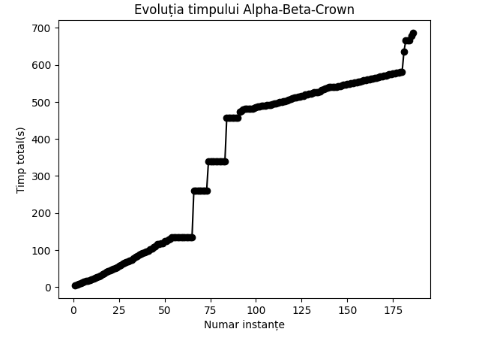
\includegraphics[]{timp_ab.png}
\section{Concluzii}
În urma verificării setului de date Acas Xu utilizând cele două tool-uri alese, Alpha-Beta-Crown și Nnenum, am obținut
rezultate satisfăcătaore în raport cu cele oficiale din cadrul competiției.

\newpage
\bibliographystyle{plain}
\bibliography{ref}

\end{document}
